\textbf{COLUNI 2018 -- Questão 32}\par\medskip Durante a organização de uma sala de materiais geográficos, os estudantes de uma escola encontraram um mapa representando um dos biomas mundiais que está destacado. Como estava sem título e sem legenda, os estudantes passaram a discutir a qual bioma o mapa corresponderia. Observe a imagem abaixo:

\par

% COLUNI-AUTO-FIGURES-BEGIN
\begin{figure}[htbp]
\centering
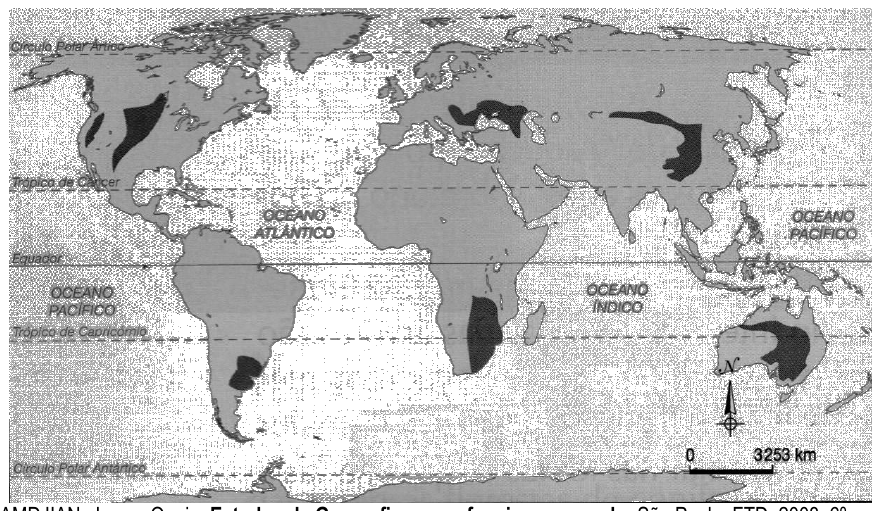
\includegraphics[width=0.95\linewidth]{static/simulados/coluni/figuras/2018/questao-32/figura-1.png}
\end{figure}
% COLUNI-AUTO-FIGURES-END

(Fonte: TAMDJIAN, James Onnig. \textbf{Estudos de Geografia: como funciona o mundo}. São Paulo: FTD, 2008. 6º ano, p. 216.)

\par

Assinale a alternativa que apresenta CORRETAMENTE o título do mapa:


\begin{enumerate}
\item Áreas originais de ocorrência de floresta equatorial.
\item Áreas originais de ocorrência de savana.
\item Áreas de ocorrência de desertos.
\item Áreas originais de ocorrência de campos.\end{enumerate}
